% Opsætter KU Tex dokument
%%%%%%%%%%%%%%%%%%%%%%%%%%%%%%%%%%%%%%%%%%%%%%%%%%%%%%%%%%%%%%%%%%%%%%%%%%%%%%%%
\documentclass{article}                                                        %
\usepackage[a4paper, hmargin={2.8cm, 2.8cm}, vmargin={2.5cm, 2.5cm}]{geometry} %
\usepackage{eso-pic}  % \AddToShipoutPicture                                   %
\usepackage{graphicx} % \includegraphics                                       %
\usepackage{subfig}                                                            %
%%%%%%%%%%%%%%%%%%%%%%%%%%%%%%%%%%%%%%%%%%%%%%%%%%%%%%%%%%%%%%%%%%%%%%%%%%%%%%%%

% Pakker til skrifttyper, tekst osv.
%%%%%%%%%%%%%%%%%%%%%%%%%%%%%%%%%%%%%%%%%%%%%%%%%%%%%%%%%%%%%%%%%%%%%%%%%%%%%%%%
    \usepackage[utf8]{inputenc}  % Implementere Unicode                        %
    \usepackage[T1]{fontenc}     % Unicode skrifttype fx. é skrives som 1 tegn %
    \usepackage[danish]{babel}   % Dansk Ordbog                                %
    \usepackage{microtype}       % Forbedre linjeombrydningen                  %
    \usepackage{libertine}       % Skrifttype                                  %
%%%%%%%%%%%%%%%%%%%%%%%%%%%%%%%%%%%%%%%%%%%%%%%%%%%%%%%%%%%%%%%%%%%%%%%%%%%%%%%%

% Pakker til matematik og kode.
%%%%%%%%%%%%%%%%%%%%%%%%%%%%%%%%%%%%%%%%%%%%%%%%%%%%%%%%%%%%%%%%%%%%%%%%%%%%%%%%
    \usepackage{mathtools}       % Udvidelse til amsmath pakken                %
    \usepackage{amsthm}          % Pakke til bevisførelse                      %
    \usepackage{amssymb}         % Extra matematiske symboler                  %
%%%%%%%%%%%%%%%%%%%%%%%%%%%%%%%%%%%%%%%%%%%%%%%%%%%%%%%%%%%%%%%%%%%%%%%%%%%%%%%%

% Pakker til layout.
%%%%%%%%%%%%%%%%%%%%%%%%%%%%%%%%%%%%%%%%%%%%%%%%%%%%%%%%%%%%%%%%%%%%%%%%%%%%%%%%
    \usepackage{fancyhdr}            % Gør det muligt at bruge sidehoveder     %
    \usepackage{graphicx}            % Mulighed for bl.a. \includegraphics     %
    \usepackage{colortbl}            % Hvis man vil farvelægge sine tabeller   %
    \usepackage{array}               % Gør miljøerne array og tabular bedre    %
    \usepackage{parskip}             % Første paragraf i afsnit indrykkes ikke %
    \usepackage{titlesec}            % Tilpassing af afstand mellem sektioner  %
    \usepackage[lastpage,user]{zref} % Side x af y                             %
%%%%%%%%%%%%%%%%%%%%%%%%%%%%%%%%%%%%%%%%%%%%%%%%%%%%%%%%%%%%%%%%%%%%%%%%%%%%%%%%


% Implementerer en række makroer og de pakker der er importeret
%%%%%%%%%%%%%%%%%%%%%%%%%%%%%%%%%%%%%%%%%%%%%%%%%%%%%%%%%%%%%%%%%%%%%%%%%%%%%%%%
    \pagestyle{fancy}                        % Implementerer sidehoved         %
    \lhead{Gymnasietjenesten}                % Venstre sidehoved               %
    \rhead{DIKU}                             % Højre sidehoved                 %
    \cfoot{\thepage\ of \zpageref{LastPage}} % Side x af y                     %
    \newtheorem*{prp}{Propostion}            % Skaber nyt theorem              %
%%%%%%%%%%%%%%%%%%%%%%%%%%%%%%%%%%%%%%%%%%%%%%%%%%%%%%%%%%%%%%%%%%%%%%%%%%%%%%%%

% Mindsker afstanden mellem sektioner
%%%%%%%%%%%%%%%%%%%%%%%%%%%%%%%%%%%%%%%%%%%%%%%%%%%%%%%%%%%%%%%%%%%%%%%%%%%%%%%%%%
\titlespacing\section{0pt}{12pt plus 4pt minus 2pt}{0pt plus 1pt minus 3pt}      %
\titlespacing\subsection{0pt}{12pt plus 4pt minus 2pt}{0pt plus 1pt minus 3pt}   %
\titlespacing\subsubsection{0pt}{12pt plus 4pt minus 2pt}{0pt plus 1pt minus 3pt}%
%%%%%%%%%%%%%%%%%%%%%%%%%%%%%%%%%%%%%%%%%%%%%%%%%%%%%%%%%%%%%%%%%%%%%%%%%%%%%%%%%%

% Laver titel
%%%%%%%%%%%%%%%%%%%%%%%%%%%%%%%%%%%%%%%%%%%%%%%%%%%%%%%%%%%%%%%%%%%%%%%%%%%%%%%%
    \title{                                                                    %
      \vspace{13em}                                                            %
      \Large{Datalogisk Institut Københavns Universitet} \\                    %
      \Huge{Latex Demo}                                                        %
    }                                                                          %                                                                              
    \author{                                                                   %
      \Large{Arinbjørn Brandsson} - \texttt{Arbr@di.ku.dk} \\                  %
      \Large{Benjamin Rotendahl} - \texttt{Bero@di.ku.dk} \\                   %
      \Large{Mathias Fleig Mortensen} - \texttt{Mamo@di.ku.dk}                 %
    }                                                                          %
    \date{                                                                     %
        \vspace{22em}                                                          %
        \today                                                                 %
    }                                                                          %
%%%%%%%%%%%%%%%%%%%%%%%%%%%%%%%%%%%%%%%%%%%%%%%%%%%%%%%%%%%%%%%%%%%%%%%%%%%%%%%%

%%%%%%%%%%%%%%%%%%%%%%%%%%%%%%%%%%%%%%%%%%%%%%%%%%%%%%%%%%%%%%%%%%%%%%%%%%%%%%%%
%%%%%%%%%%%%%%%%%%%%      Her starter dokumentet    %%%%%%%%%%%%%%%%%%%%%%%%%%%%
\begin{document}

% KU forside
%%%%%%%%%%%%%%%%%%%%%%%%%%%%%%%%%%%%%%%%%%%%%%%%%%%%%%%%%%%%%%%%%%%%%%%%%%%%%%%%%
    \AddToShipoutPicture*{\put(0,0){\includegraphics*[viewport=0 0 700 600]     %
    {include/ku-farve}}}                                                        %
    \AddToShipoutPicture*{\put(0,602){\includegraphics*[viewport=0 600 700 1600]%
    {include/natbio-farve}}}                                                    %
    \AddToShipoutPicture*{\put(0,0){\includegraphics*{include/nat-en}}}         %
    \clearpage                                                                  %
%%%%%%%%%%%%%%%%%%%%%%%%%%%%%%%%%%%%%%%%%%%%%%%%%%%%%%%%%%%%%%%%%%%%%%%%%%%%%%%%%

%Disse linjer skaber forside, evt indholdsfortegnelse, og sætter sidetal
%%%%%%%%%%%%%%%%%%%%%%%%%%%%%%%%%%%%%%%%%%%%%%%%%%%%%%%%%%%%%%%%%%%%%%%%%%%%%%%%
    \maketitle              % Forside                                          %
    \thispagestyle{empty}   % Fjerner sidetal forside                          %
        % Slå disse til hvis der ønskes indholdsfortegnelse                    %
        %%%%%%%%%%%%%%%%%%%%%%%%%%%%%%%%%%%%%%%%%%%%%%%%%%%%%%%%%%%%%%%%%%%%%%%%
           % TODO2 Hvorfor skal den køres to gange?   
            \newpage                % Side til indholdsfortegnelse            %
            \thispagestyle{empty}   % Fjerner sidetal fra indholdsfortegnelse %
            \tableofcontents        % Skaber indholdsfortegnelse              %
        %%%%%%%%%%%%%%%%%%%%%%%%%%%%%%%%%%%%%%%%%%%%%%%%%%%%%%%%%%%%%%%%%%%%%%%%
    \newpage                % Første rigtige side
    \setcounter{page}{1}    % Sætter rigtigt sidetal på første side
%%%%%%%%%%%%%%%%%%%%%%%%%%%%%%%%%%%%%%%%%%%%%%%%%%%%%%%%%%%%%%%%%%%%%%%%%%%%%

% TODO1 Lav sektion 
\section{Abstract}
Cras justo odio, dapibus ac facilisis in, egestas eget quam. Nullam id dolor id nibh ultricies vehicula ut id elit. Cum sociis natoque penatibus et magnis dis parturient montes, nascetur ridiculus mus. Etiam porta sem malesuada magna mollis euismod. Curabitur blandit tempus porttitor. Maecenas sed diam eget risus varius blandit sit amet non magna. Sed posuere consectetur est at lobortis.

Lorem ipsum dolor sit amet, consectetur adipiscing elit. Aenean lacinia bibendum nulla sed consectetur. Aenean eu leo quam. Pellentesque ornare sem lacinia quam venenatis vestibulum. Aenean lacinia bibendum nulla sed consectetur.

Donec ullamcorper nulla non metus auctor fringilla. Maecenas faucibus mollis interdum. Cras mattis consectetur purus sit amet fermentum. Maecenas faucibus mollis interdum.


\section{Pæn Kode}

\section{Introduktion}
    Dette dokument er lavet til de gymnasieelever, der er tilmeldt
    SRP-/databehandlings workshop på Datalogisk Institut Københavns Universitet.
    Vi glæder os meget til at få jer på besøg. Denne PDF indeholder praktisk
    information og en installationsguide. For at vi kan få en rigtig god
    dag sammen, vil vi gerne bede jer om at installere nogle programmer på jeres computere, 
    så I er klar til at lære LaTeX fra starten.





\section{Praktisk information}
    Workshoppen finder sted i HCØ bygningen, hvor der vil være forelæsning i
    auditorium 10 og øvelser i de omliggende  lokaler.     
    
    Adressen er Universitetsparken 5, 2100 København.
    Op til kl 10.00 vil der være en til at tage imod, og vise jer hen til
    auditoriet ved indgangen markeret på kortet.

    \subsection{Program for mandag}
    \begin{description}
        \item[kl 10.00-12.00] | Velkomst og forelæsning \\        
        Vi starter med velkomst og en forelæsning om LaTeX.
        Forelæsningen vil give en introduktion til hvad LaTeX er, hvordan det
        fungerer, og hvilke fordele det har over programmer som Word.
        
        \item[kl 12.00-12.45] | Pause ~ \\
        Til frokost kan i enten have madpakke med, eller tage penge med til
        kantinen.

        \item[12.45 - 15.00] | Øvelser ~ \\
        Til øvelserne vil i blive givet et print lavet i LaTeX med forskellige
        formler, tabeller, og figurer. Jeres opgave vil så være at genskabe
        dette dokument i LaTeX. Vi samler op med en gennemgang på projektoren.
    \end{description}



    \subsection{Program for tirsdag}
    \begin{description}
        \item[kl 10.00-12.00] | Opsamling fra mandag og øvelser ~ \\
        Tirsdag vil vi starte med at vise, hvordan LaTeX brillerer særligt
        ved større rapporter. Herefter vil vi gerne bede jer om at tage en af
        jeres egne afleveringer med, som i så skal ``TeXe''.

        \item[kl 12.00-12.45] | Pause ~ \\
        Til frokost kan i enten have madpakke med, eller tage penge med til
        kantinen.

        \item[12.45 - 15.00] | Intro til databehandling ~ \\
        Vi vil holde en forelæsning, hvor vi demonstrerer forskellige databehandlings
        værktøjer, samt hvordan de sammenarbejder med LaTeX.
        
        \item Øl på cafeen? 
        % TODO spørg vejl
    \end{description}
 
% TODO Lav nye linjer, mellemrum, opbygning og god tex stil, fejlhåndtering
% Reseverede ord,


\section{Matematik}
% flalign, $$, _, ^, {}, græske bogstaver
Man kan finde rødder i en andengradsligning af formen $ax^2 + bx + c = 0$ sådan her.
$$
	\frac{-b \pm \sqrt{b^2 - 4ac}}{2a} 
$$

\begin{flalign*}
	E &= MC^2 \\
	ax^2 + bx + c &= 0 \\
	\frac{N!}{(N-0)!0!} \leq 1 + 1  \\
\end{flalign*}

\section{tabeller}
\begin{center}
  \begin{tabular}{| l | c || c | }
    \hline
    1 & 2 & $p = np$ \\ \hline
    4 & 5 & 6 \\ \hline
    7 & 8 & 9 \\
        7 & 8 & 9 \\
            7 & 8 & 9 \\
                7 & 8 & 9 \\ 	\hline 
        7 & 8 & 9 \\ 
                        7 & 8 & 9 \\
                            7 & 8 & 9 \\
                                7 & 8 & 9 \\
    \hline
  \end{tabular}
\end{center}







\section{lister}
\begin{itemize}
	\item Guld tuborg
	
	\item kridt 
	
	\item Arinbjørn
\end{itemize}


\begin{description}
	\item[En god øl] Guld tuborg
	
	\item[noget at tegne med] kridt 
	
	\item[dude med skæg] Arinbjørn
\end{description}


\begin{enumerate}
	\item Guld tuborg
	
	\item kridt 
	
	\item Arinbjørn
\end{enumerate}

\section{}

$$
\left(
	\begin{array}{c}
	n \\
	i 
	\end{array}
\right)
$$

\section{Figurer}
\begin{figure}[h!]
    \centering
    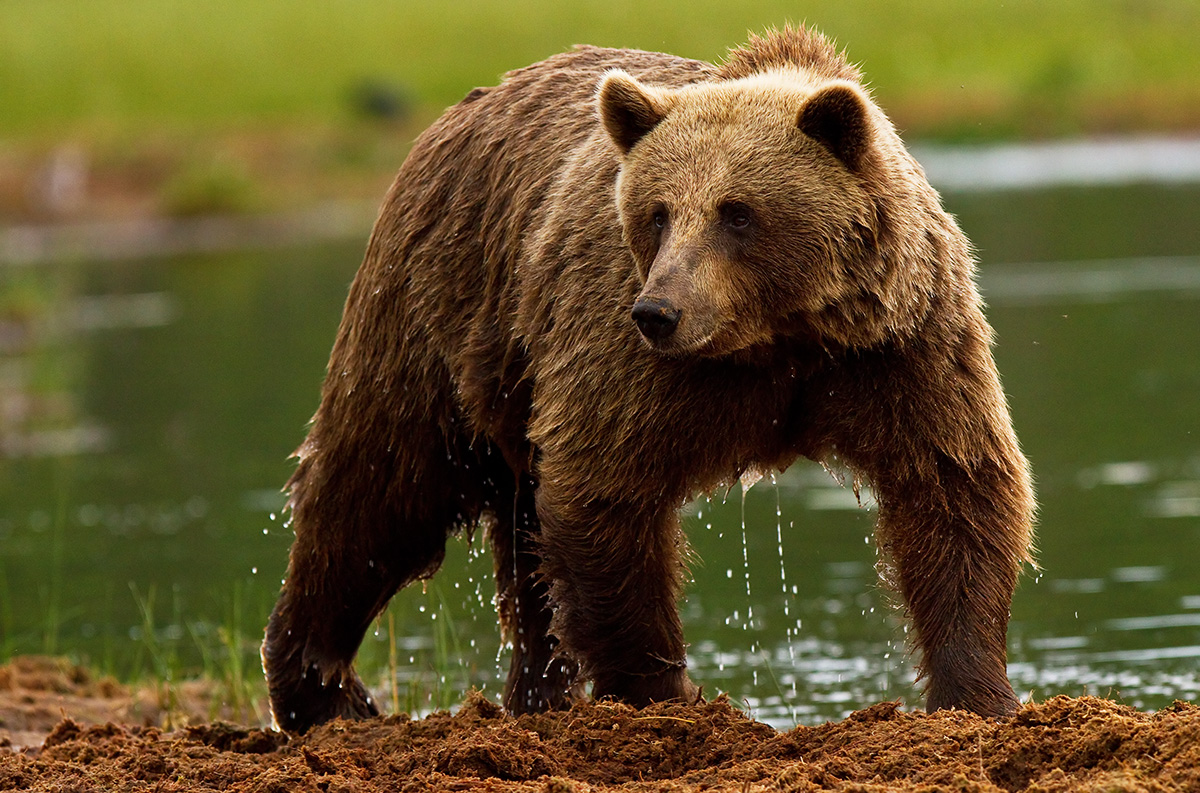
\includegraphics[width=0.5\textwidth]{bear.jpg}
    \caption{Brøl}
\end{figure}

\end{document}
